\section{DTN7}

\subsection{Other DTN7 Components}

\begin{frame}
  \frametitle{Other DTN7 Components}

  \begin{itemize}
  \item Store for Bundles that are waiting for delivery
  \item RESTful API to dispatch and fetch Bundles
  \item Peer Discovery to detect nearby nodes
  \end{itemize}
\end{frame}

\subsection{DTN7 Programs}

\begin{frame}[fragile]
  \frametitle{DTN7 Programs}

  \begin{itemize}
  \item \texttt{dtnd}: \acs{DTN} daemon
  \item \texttt{dtncat}: command line tool
  \end{itemize}

  \begin{figure}
    \lstset{
      basicstyle=\ttfamily\scriptsize,
      commentstyle=\color{gray},
      language=sh,
    }

    \begin{lstlisting}
# Sending a Bundle
$ dtncat send http://localhost:8080/ dtn:sink/lux <<< "3782 lx"

# Retrieving a received Bundle
$ dtncat fetch http://localhost:8080/
    \end{lstlisting}
  \end{figure}
\end{frame}

\subsection{DTN7 Architecture}

\begin{frame}
  \frametitle{DTN7 Architecture}

  \begin{figure}
    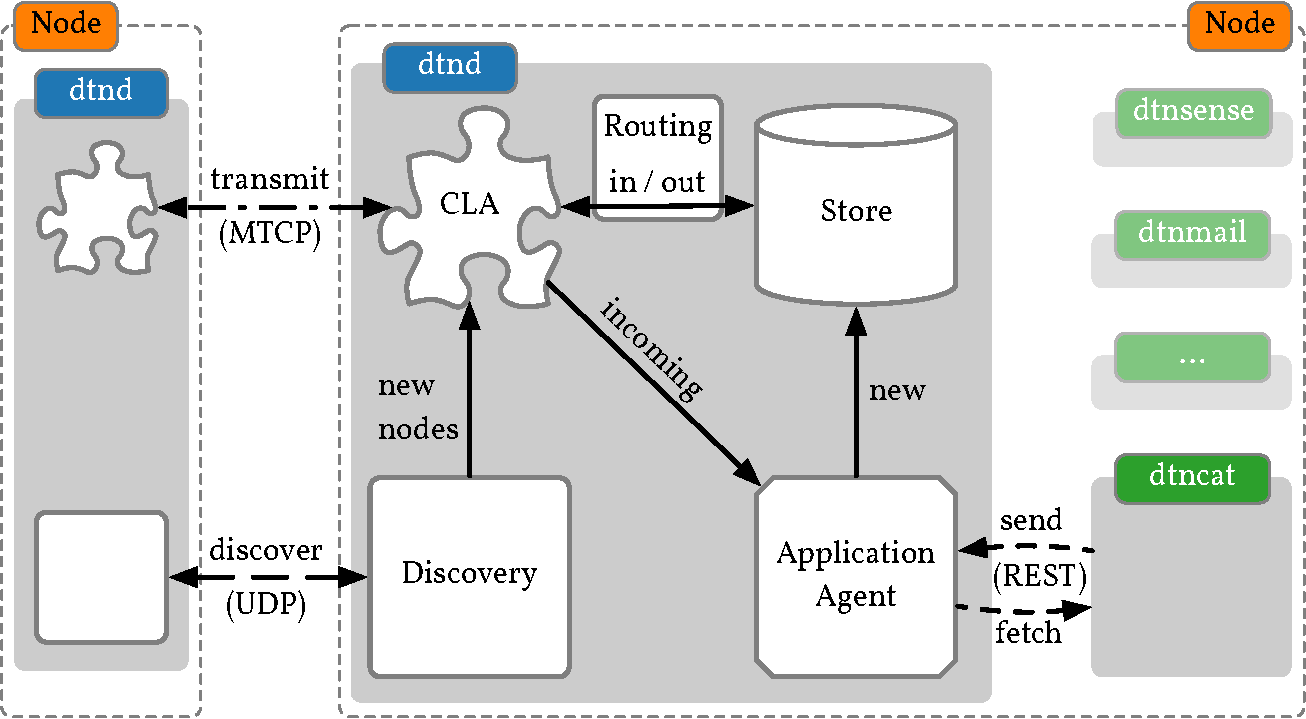
\includegraphics[width=0.9\linewidth,keepaspectratio]{include/dtn7-architecture}
  \end{figure}
\end{frame}
